\chapter{ระเบียบวิธีดำเนินโครงงาน}
\label{Ch:Methodology}

วิธีการเพิ่มรูปภาพและอ้างอิงไปยังรูปภาพ \ref{fig:example_figure}

\begin{figure}[h]
    \centering
    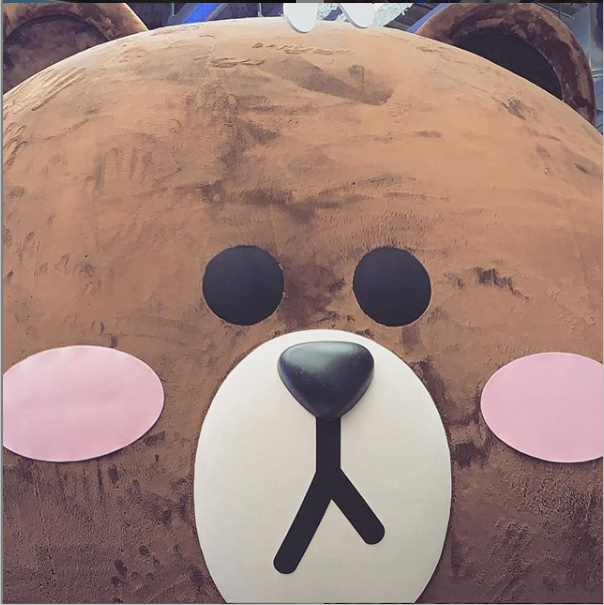
\includegraphics[scale = 0.5]{figures/chap2/Sample101.PNG}
    \captionsetup{name = รูป}
    \caption{คำอธิบายรูปภาพ}
    \label{fig:example_figure}
\end{figure}

วิธีการเพิ่ม{\boldfont สมการ} และ{\italicfont อ้างอิง}ไปยังสมการ \ref{eq:example_equation}.

\begin{equation} 
y = \sqrt{x^2+1}
\label{eq:example_equation}
\end{equation}